\begin{figure}[!htb]
    \centering
    % \begin{adjustbox}{minipage=\linewidth,scale=0.7}
    \Subfigure[0.3]{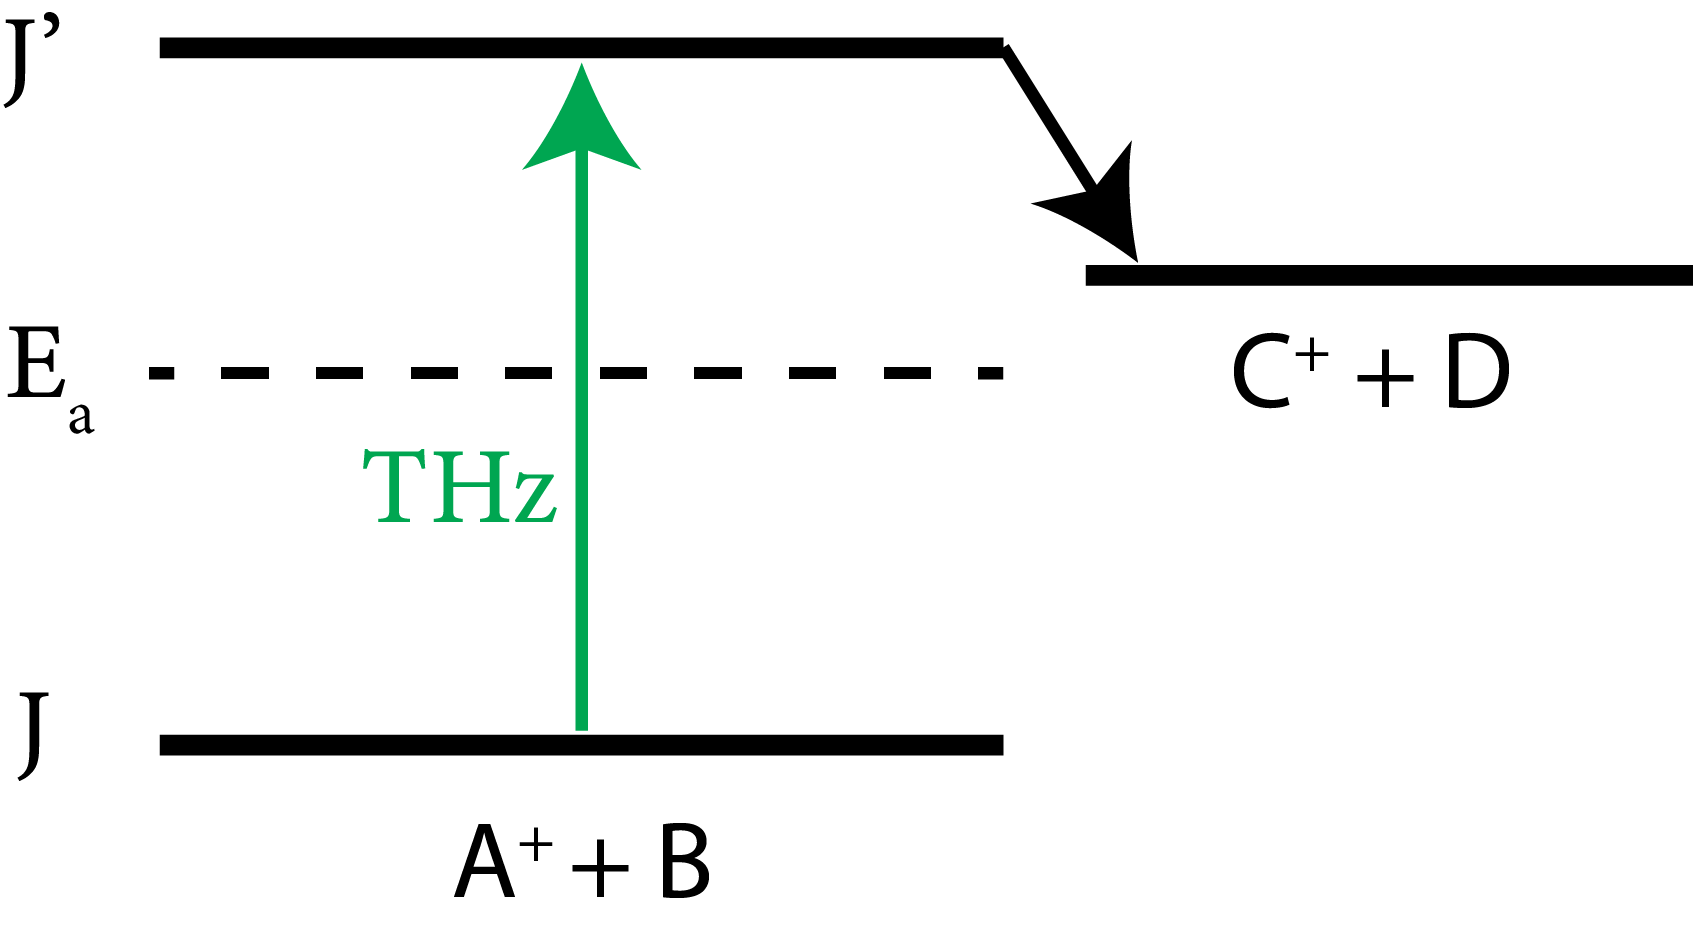
\includegraphics[width=1\textwidth]{figures/intro/rotational-action/LIR.png}}{LIR}{\label{fig:action:methods:rotational:LIR}}
    \hfill
    \Subfigure[0.3]{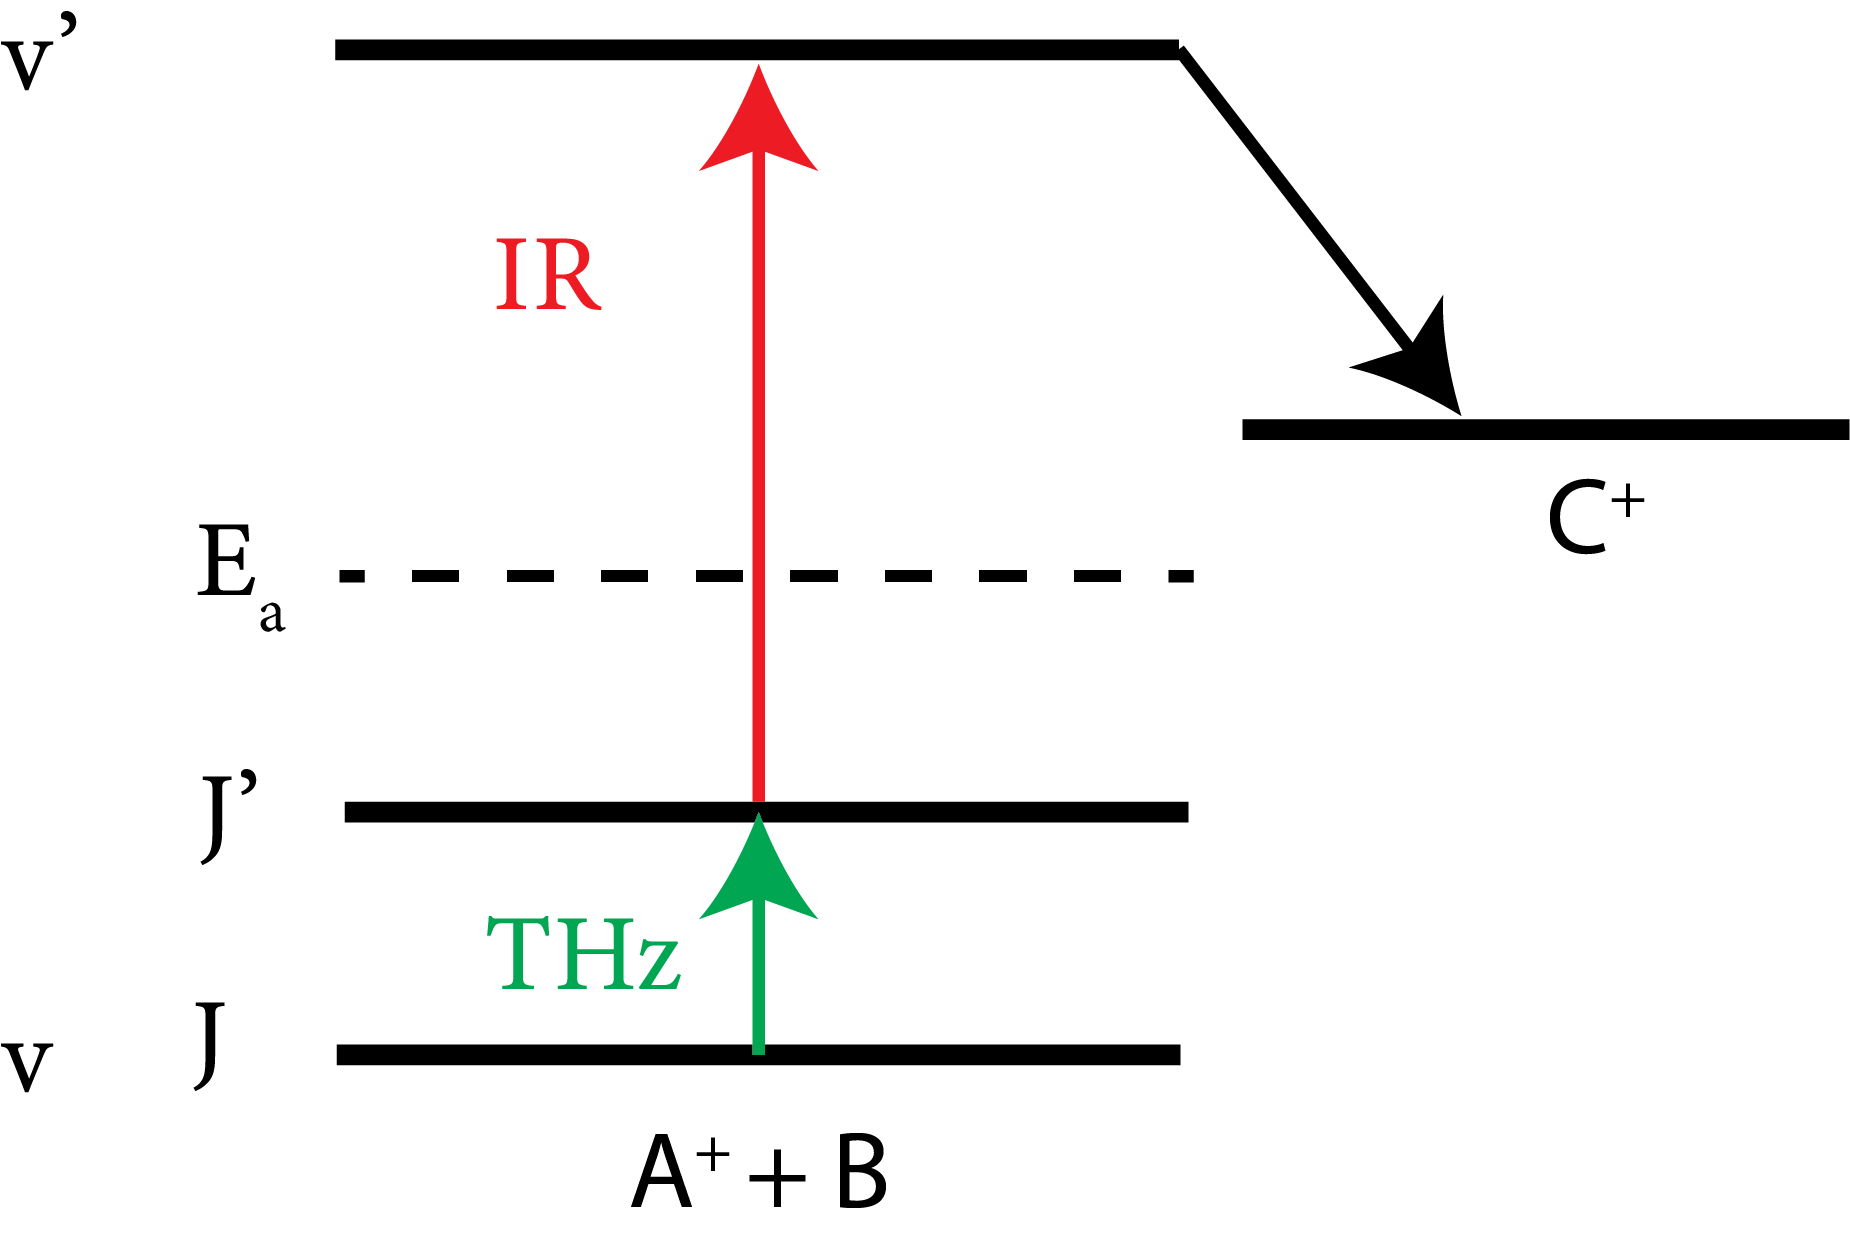
\includegraphics[width=1\textwidth]{figures/intro/rotational-action/DR_LIR.png}}{DR \emph{via} LIR}{\label{fig:action:methods:rotational:DR_LIR}}
    \hfill
    \Subfigure[0.3]{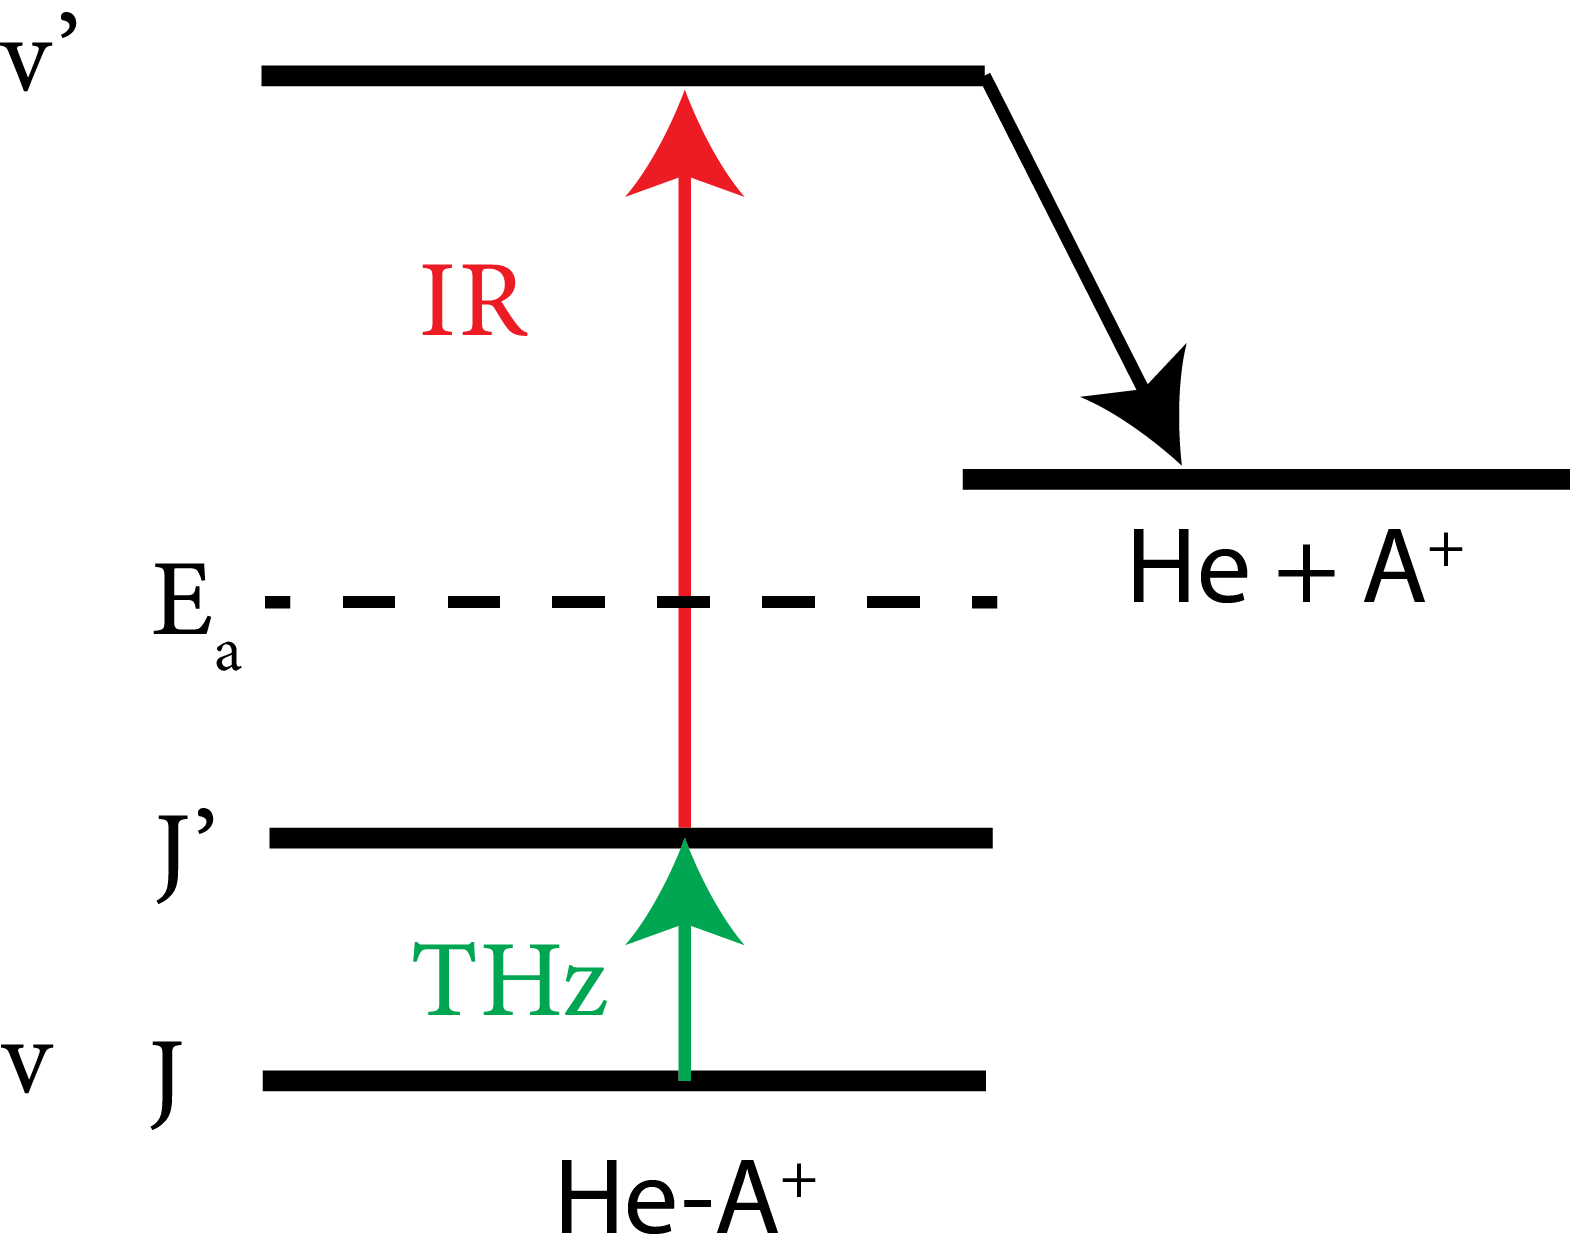
\includegraphics[width=1\textwidth]{figures/intro/rotational-action/DR_THz-IRPD.png}}{DR \emph{via} predis.}{\label{fig:action:methods:rotational:DR_THz_IR}}
    \hfill
    
    \hfill
    
    \Subfigure[0.3]{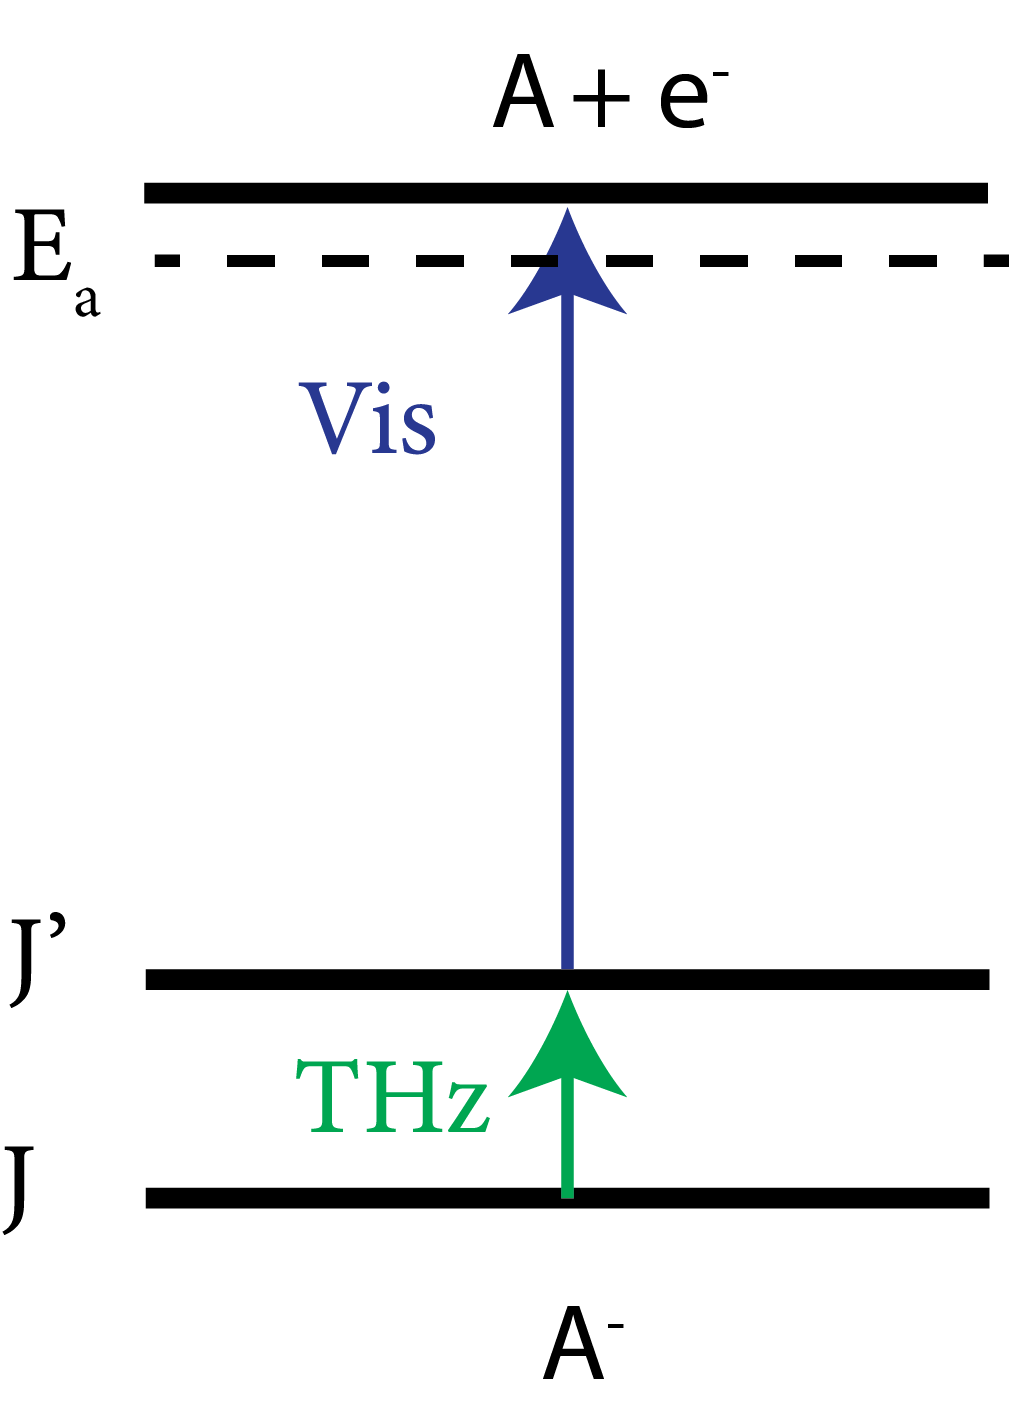
\includegraphics[scale=0.3]{figures/intro/rotational-action/EA.png}}{DR \emph{via} \emph{e}$^-$ det.}{\label{fig:action:methods:rotational:DR_THz_Vis}}
    \hfill
    \Subfigure[0.3]{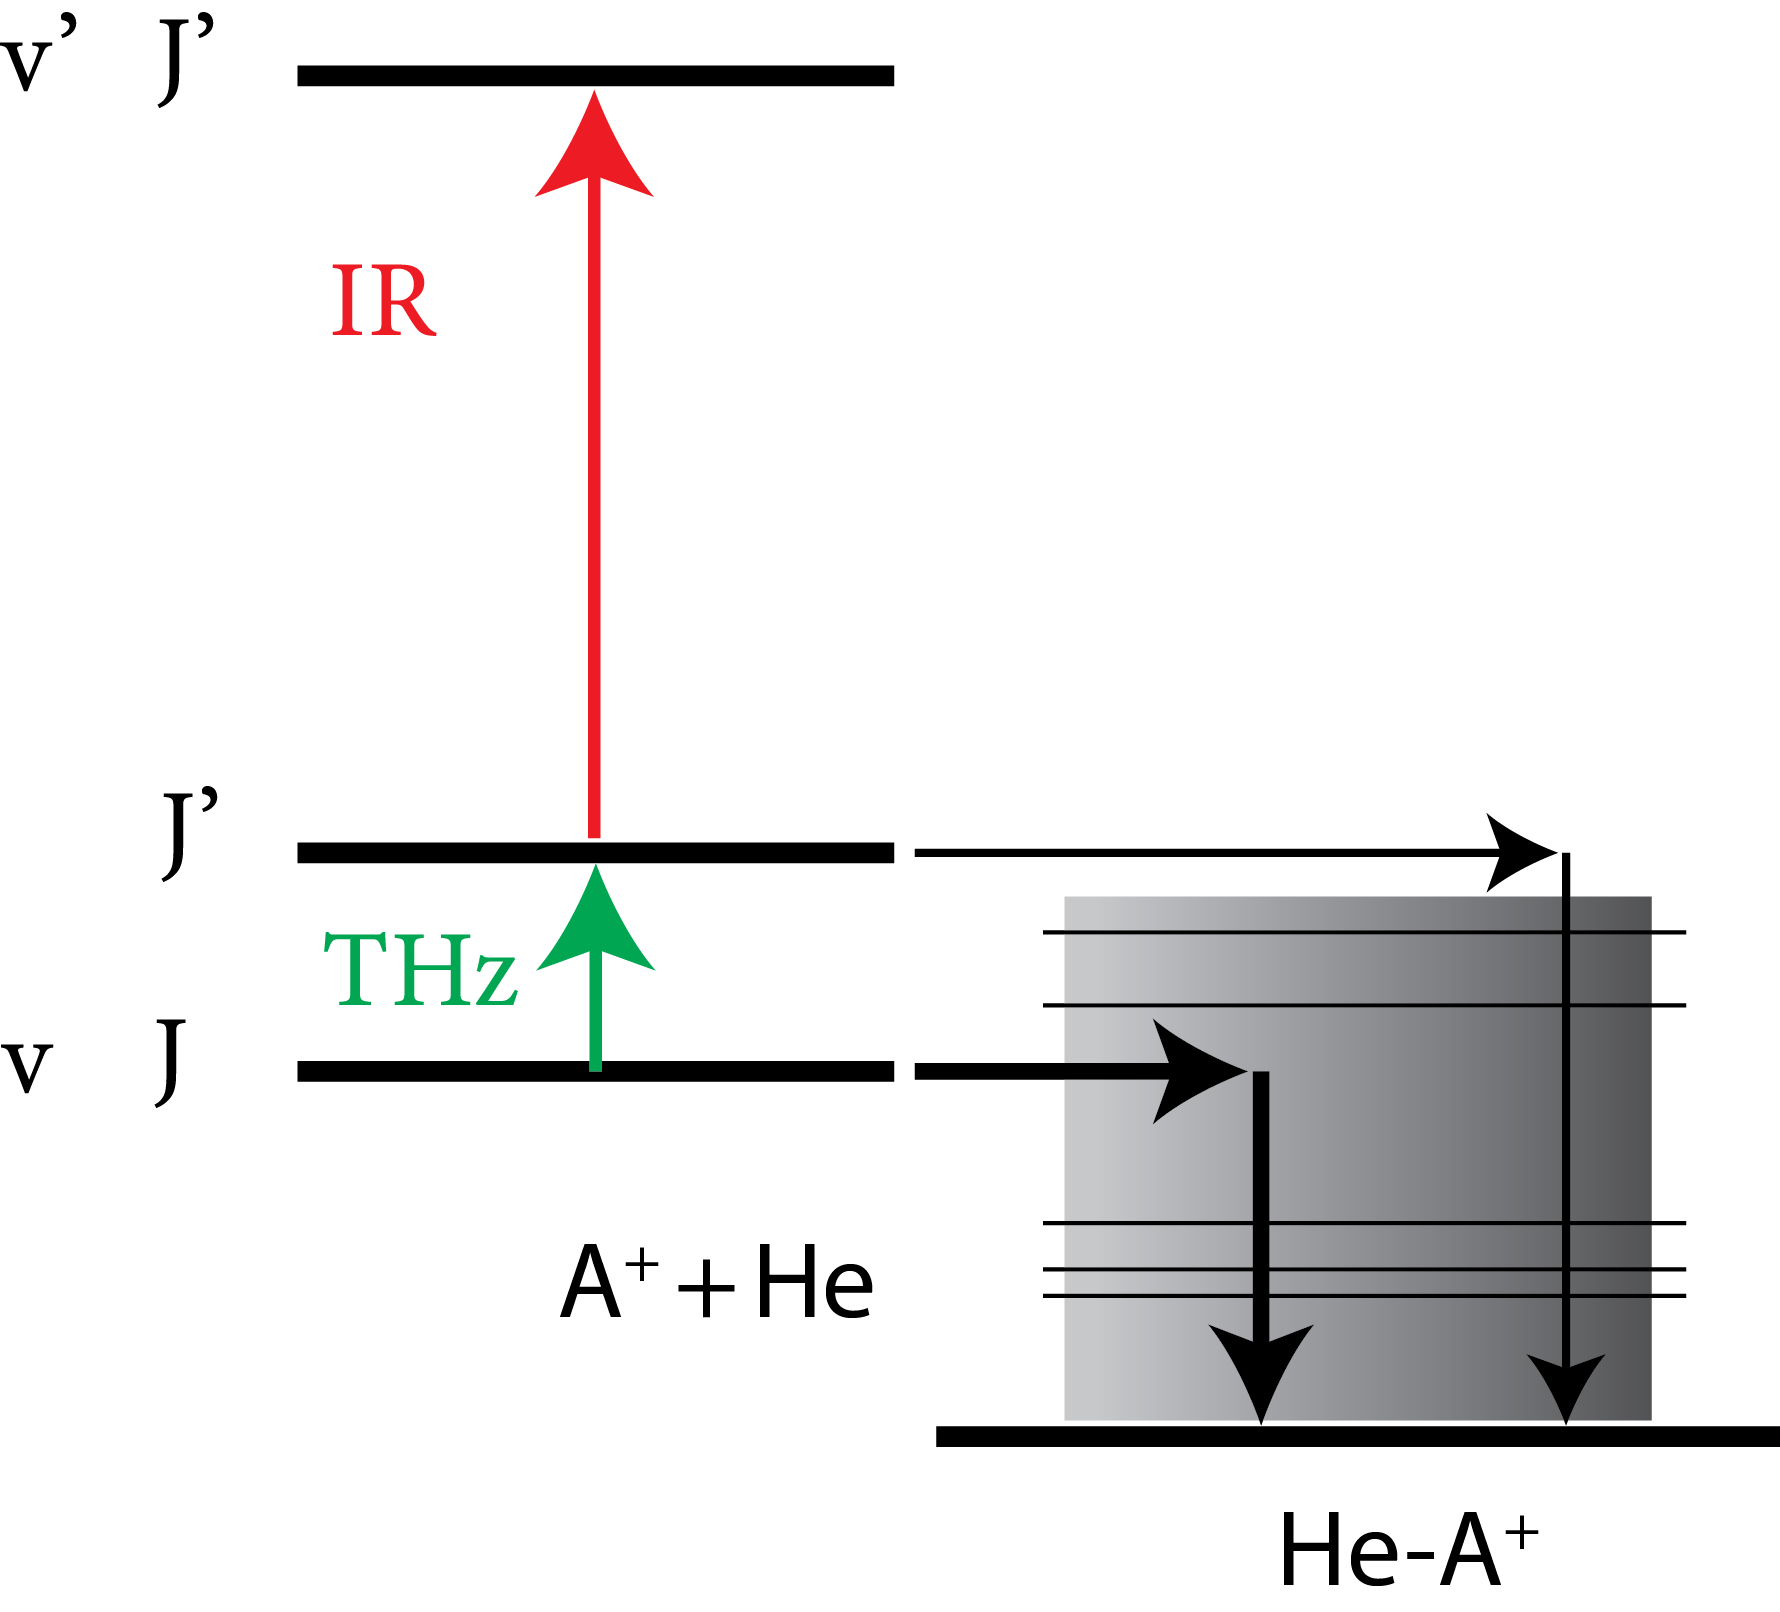
\includegraphics[width=1\textwidth]{figures/intro/rotational-action/DR_THz_IR_LIICG.png}}{DR \emph{via} LIICG}{\label{fig:action:methods:rotational:DR_THz_IR_LIICG}}
    \hfill
    \Subfigure[0.3]{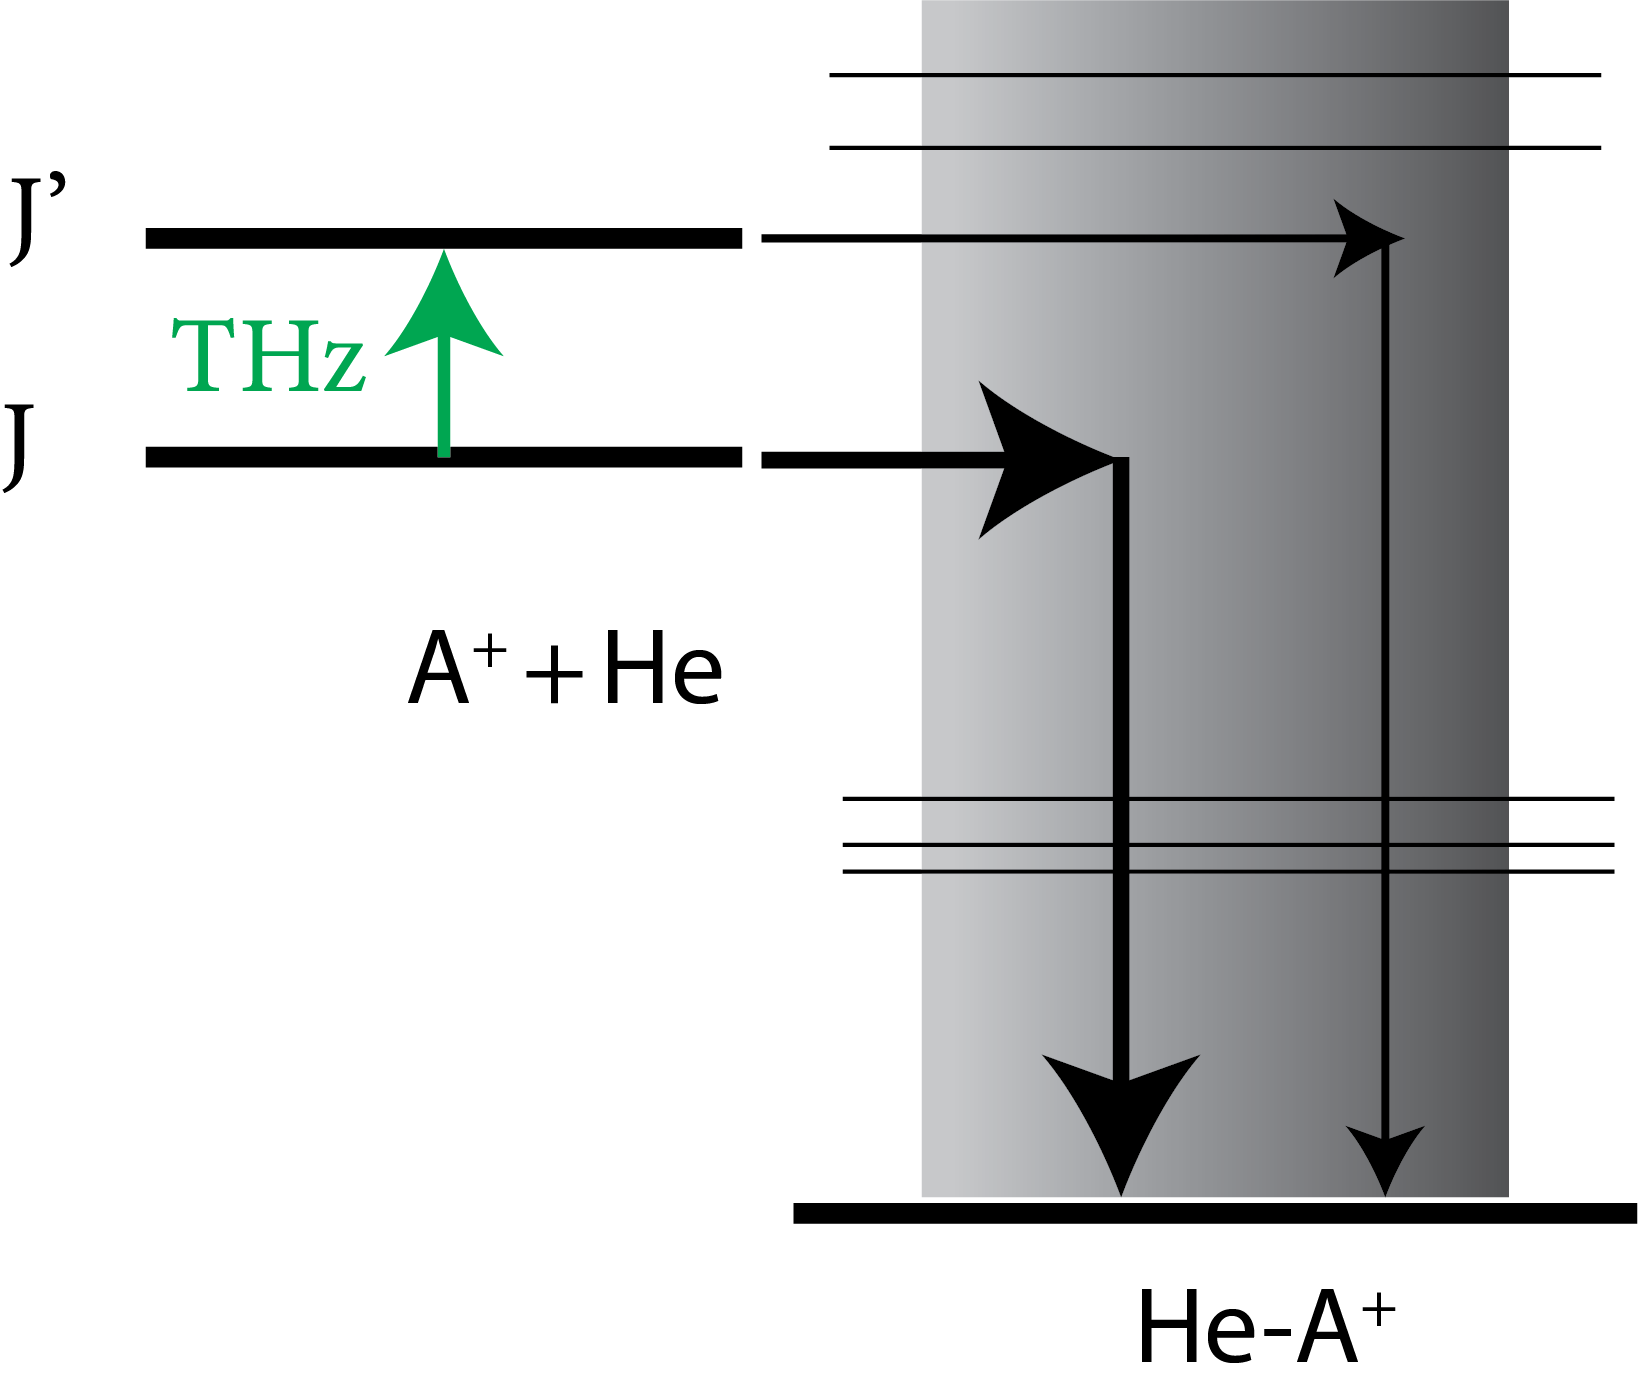
\includegraphics[width=1\textwidth]{figures/intro/rotational-action/ROSAA.png}}{ROSAA}{\label{fig:action:methods:rotational:ROSAA}}
    % \hfill
    % \end{adjustbox}
    \caption{Schematic diagrams of rotational action spectroscopic methods. The captions indicate the corresponding name of the method. DR stands for double resonance. \qt{predis.} and \qt{det.} in (c) and (d) correspond to \qt{predissociation} and \qt{detachment}, respectively. The symbol A and B indicates molecular species while superscript (such as A$^+$) indicates molecular cations. He indicates a helium atom while He-A$^+$ indicates a weakly bound helium-ion complex.}
    \label{fig:action:methods:rotational}
\end{figure}
\clearpage
